% Kompilasi dengan XeLaTeX: latexmk -xelatex 2026-10-22-machine-learning.tex
% Penjelasan machine learning Wind Edge Chip untuk persiapan QnA Demo Day (23 Okt 2026).
% Semua angka berasal dari ml/results/*.json, dashboard/wec/model_bundle.json, dan tes di dashboard/wec/test/.
\documentclass[10.5pt,a4paper]{article}

\usepackage[indonesian]{babel}
\usepackage{fontspec}
\IfFontExistsTF{Calibri}{\setmainfont{Calibri}}{\setmainfont{Carlito}}
\setmonofont{DejaVu Sans Mono}[Scale=0.82]
\usepackage[margin=2cm]{geometry}
\usepackage{microtype}
\usepackage{xcolor}
\usepackage{graphicx}
\usepackage{tikz}
\usetikzlibrary{positioning,fit,backgrounds,arrows.meta,calc}
\usepackage{booktabs,tabularx,array,longtable}
\usepackage{enumitem}
\usepackage[most]{tcolorbox}
\usepackage[hidelinks]{hyperref}
\usepackage{titlesec}
\usepackage{amsmath}

% Gaya bersama diagram (dipakai laporan progress dan deck). Warna anggota sama dengan jobdesc.tex.
\providecolor{izma}{RGB}{31,94,170}
\providecolor{genis}{RGB}{40,130,70}
\providecolor{alif}{RGB}{190,90,20}
\providecolor{shania}{RGB}{140,60,150}
\providecolor{lama}{RGB}{110,110,110}
\providecolor{merah}{RGB}{185,40,40}
\tikzset{
  kotak/.style={draw, rounded corners=3pt, align=center, font=\footnotesize, inner sep=4pt, line width=0.8pt, minimum height=0.9cm},
  milik/.style={kotak, draw=#1, fill=#1!10},
  abu/.style={kotak, draw=lama, fill=black!4},
  panah/.style={-{Stealth[length=2mm]}, line width=0.7pt, draw=black!70},
  putus/.style={panah, dashed},
  label/.style={font=\scriptsize\itshape, text=black!70, fill=white, inner sep=1pt},
  wadah/.style={draw=#1!60, fill=#1!4, rounded corners=5pt, line width=0.6pt, inner sep=6pt},
}

\newcommand{\cmd}[1]{\texttt{#1}}
\titleformat{\section}{\large\bfseries\color{izma}}{\thesection.}{0.5em}{}
\titleformat{\subsection}{\normalsize\bfseries}{\thesubsection}{0.5em}{}
\setlist{nosep, leftmargin=1.4em}
\setlength{\parindent}{0pt}
\setlength{\parskip}{4pt}
\newtcolorbox{ringkas}[1][]{colback=izma!5, colframe=izma, boxrule=0.8pt, arc=3pt, left=6pt, right=6pt, top=4pt, bottom=4pt, fonttitle=\bfseries, title={#1}}
\newtcolorbox{perhatian}[1][]{colback=merah!5, colframe=merah!80!black, boxrule=0.8pt, arc=3pt, left=6pt, right=6pt, top=4pt, bottom=4pt, fonttitle=\bfseries, title={#1}}
\newtcolorbox{jawab}[1][]{colback=genis!5, colframe=genis, boxrule=0.6pt, arc=2pt, left=5pt, right=5pt, top=3pt, bottom=3pt, fonttitle=\bfseries\small, title={#1}}

\begin{document}
\sloppy\setlength{\emergencystretch}{3em}

\begin{center}
{\LARGE\bfseries Machine Learning Wind Edge Chip}\\[3pt]
{\large Penjelasan lengkap dan bahan QnA Demo Day}\\[2pt]
{\normalsize Tim Chitato \textbullet{} DeepTech for Smart-X Hackathon 2026 \textbullet{} Kamis 22 Oktober 2026 malam \textbullet{} Izma Alhazmi Herdian}
\end{center}

\begin{ringkas}[Ringkasan satu halaman]
\begin{itemize}
  \item \textbf{Untuk apa:} membantu pemilik turbin memutuskan energi tanpa menebak. Ada tiga tugas: (1) \textbf{prediksi rata-rata daya 1 jam ke depan},
        (2) \textbf{status turbin} dari kurva daya wajar, (3) \textbf{aki 1 jam ke depan} (simulasi aki 12 V 50 Ah).
  \item \textbf{Data apa:} data live turbin atap Gedung CRIMSE ITB (daya PZEM, angin dan cuaca stasiun) lewat Raspberry Pi $\to$ MQTT,
        ditambah \textbf{prakiraan angin Open-Meteo}. Model dilatih dari \textbf{181.228 menit} data nyata (30 Mar--20 Okt 2026).
  \item \textbf{Model apa:} jaringan saraf kecil \textbf{MLP 16-32-16-1} dengan bilangan bulat 8-bit (\textbf{INT8}), dilatih langsung dengan
        aritmetika chip (QAT). Bobot yang sama persis dijalankan di Node-RED, ESP32, dan \textbf{chip FPGA} Tang Nano 4K.
  \item \textbf{Seberapa akurat:} uji 1--20 Okt (16.255 menit, tidak dipakai melatih): galat rata-rata \textbf{MAE 5,48 W} vs persistence
        8,67 W ($-$37\%), skill +0,40. Setara model besar (Transformer: MAE 5,70 W, RMSE 10,07 W; MLP INT8: MAE 5,48 W, RMSE 10,25 W) tetapi muat di chip kecil.
  \item \textbf{Tahan gangguan:} sensor daya diam, data berlubang, internet putus, dan Raspi mati lama semuanya punya mode cadangan
        yang diuji (Bagian~\ref{sec:mode}).
  \item \textbf{Chip:} hasil chip identik bit demi bit (uji di papan 5.373/5.373), 309 siklus per prediksi, energi per prediksi
        $\approx$17$\times$ lebih kecil dari Raspberry Pi (estimasi INA219).
\end{itemize}
\end{ringkas}

\section{Gambaran besar: dari sensor sampai keputusan}
\begin{center}
\begin{tikzpicture}[node distance=0.45cm and 0.55cm, every node/.style={font=\footnotesize}]
  \node[milik=lama, text width=2.2cm] (s) {\textbf{Sensor turbin}\\PZEM-017: daya, V, I\\stasiun: angin, arah, suhu, kelembapan};
  \node[milik=genis, text width=2.0cm, right=of s] (r) {\textbf{Raspberry Pi}\\baca tiap $\pm$5 dtk\\kirim MQTT};
  \node[milik=izma, text width=2.6cm, right=of r] (n) {\textbf{Mesin ML (Node-RED)}\\ringkas per menit\\16 fitur $\to$ MLP INT8};
  \node[milik=alif, text width=2.0cm, right=of n] (c) {\textbf{Chip FPGA}\\fitur yang sama\\hasil identik};
  \node[milik=shania, text width=2.4cm, below=of n] (d) {\textbf{Dashboard}\\prediksi, status, aki, digital twin};
  \node[milik=lama, text width=2.2cm, above=of n] (o) {\textbf{Open-Meteo}\\prakiraan angin per jam};
  \node[milik=lama, text width=2.4cm, below=of r] (h) {\textbf{Riwayat cadangan}\\\texttt{WEC/state} + Google Sheets 3 jam};
  \draw[panah] (s) -- (r); \draw[panah] (r) -- (n); \draw[panah] (n) -- (c); \draw[panah] (n) -- (d); \draw[panah] (o) -- (n);
  \draw[putus] (h) -- (n); \draw[putus] (c.south) |- (d.east);
\end{tikzpicture}
\end{center}
Setiap pergantian menit, mesin ML (function node ``Mesin WEC'' di Node-RED \cmd{citaitb.com}) meringkas data menit yang baru selesai,
menghitung 16 fitur, menjalankan model, lalu mengirim hasil ke dashboard dan ke chip (lewat ESP32-S3). Model \emph{tidak} dilatih ulang
saat live: bobotnya tetap, dilatih sekali di laptop dari data historis.

\section{Data latih dan pembersihan}
\begin{tabularx}{\linewidth}{@{}l X@{}}
\toprule
Sumber & Ekspor Google Sheets ``Turbine Database'' (CSV di \cmd{data/raw/turbine-database/}) + arsip Open-Meteo \\
Periode & 30 Mar--20 Okt 2026; 2,22 juta baris mentah $\to$ \textbf{181.228 menit} berisi data (61,7\% dari seluruh menit; sisanya celah, terutama Raspi reboot) \\
Pembagian (kronologis) & latih 30 Mar--31 Jul (99.260 menit) \textbullet{} validasi Agu--Sep (31.700) \textbullet{} uji 1--20 Okt (16.255). Tidak diacak, supaya model tidak ``mengintip'' masa depan. \\
\bottomrule
\end{tabularx}

\textbf{Aturan pembersihan} (\cmd{ml/common/preprocess.py}):
\begin{itemize}
  \item Sel rusak akibat Excel (tanggal tersimpan sebagai angka $>$45.000) dibuang; 105.329 nilai daya dihitung ulang dari V$\times$I.
  \item Baris ``OFF'' (PZEM tidak terbaca) $\to$ daya \textbf{0 W}. PZEM mati saat keluaran turbin $<$7 V, yaitu saat angin lemah.
  \item Angin Arduino dibuang (macet di 1,25 m/s); dipakai angin stasiun. Angin $>$8 m/s, arah $-115$ (sentinel), suhu $<$5\,°C $\to$ kosong.
  \item Spike daya di atas batas fisik beban 35\,$\Omega$ dibuang; data diringkas per menit; celah $>$10 menit tidak diisi.
\end{itemize}

\section{Fitur 1 --- Prediksi daya 1 jam ke depan (inti)}
\subsection{Apa yang diprediksi}
Target = \textbf{rata-rata daya 60 menit ke depan} (W). Karena rata-rata selama 1 jam, angka yang sama adalah \textbf{energi (Wh) jam berikutnya}.
Contoh: prediksi 25 W berarti sekitar 25 Wh akan dihasilkan dalam satu jam ke depan.

\subsection{16 fitur (masukan model), dihitung tiap menit}
\begin{tabularx}{\linewidth}{@{}l X@{}}
\toprule
Fitur & Arti \\
\midrule
\cmd{p\_now}, \cmd{p\_lag5/15/30/60} & daya sekarang, 5, 15, 30, 60 menit lalu (pola naik/turun) \\
\cmd{p\_mean60} & rata-rata daya 60 menit terakhir \\
\cmd{w\_now}, \cmd{w\_mean10}, \cmd{w\_mean60} & angin sekarang, rata-rata 10 dan 60 menit \\
\cmd{w3\_mean10} & rata-rata angin pangkat tiga 10 menit (daya angin $\propto v^3$) \\
\cmd{dir\_sin}, \cmd{dir\_cos} & arah angin (sin/cos supaya 359° dekat dengan 1°) \\
\cmd{hour\_sin}, \cmd{hour\_cos} & jam dalam sehari (pola harian: malam tenang, sore berangin) \\
\cmd{rho} & kepadatan udara dari suhu, kelembapan, tekanan \\
\cmd{om\_wind\_next} & \textbf{rata-rata prakiraan angin Open-Meteo 60 menit ke depan} (satu-satunya fitur yang melihat masa depan) \\
\bottomrule
\end{tabularx}

\subsection{Model: MLP INT8 16-32-16-1}
\begin{center}
\begin{tikzpicture}[x=2.6cm, every node/.style={font=\footnotesize}]
  \foreach \i/\n/\t in {0/16/{16 fitur\\INT8}, 1/32/{32 neuron\\ReLU}, 2/16/{16 neuron\\ReLU}, 3/1/{1 keluaran\\$\times$0,972 W}}
    {\node[milik=izma, text width=1.8cm, minimum height=1.2cm] (L\i) at (\i,0) {\t};}
  \foreach \a/\b in {0/1,1/2,2/3} \draw[panah] (L\a) -- (L\b);
  \node[below=0.25cm of L1, text width=6cm, align=center, font=\scriptsize\itshape] {tiap lapisan: jumlah perkalian bobot $\times$ masukan + bias, lalu dibulatkan ke 0--127};
\end{tikzpicture}
\end{center}
\begin{itemize}
  \item \textbf{Kuantisasi masukan:} tiap fitur diubah ke bilangan bulat $x_q = \mathrm{clamp}(\mathrm{round}((x-c)/s), -128, 127)$ dengan pusat $c$ dan skala $s$ per fitur.
  \item \textbf{Tiap lapisan:} $y = \mathrm{clamp}\big(((\textstyle\sum w x + b)\cdot 32) \gg 8,\ 0,\ 127\big)$, sama persis dengan rangkaian \cmd{post\_process.v} di chip.
  \item \textbf{Keluaran:} bilangan 0--127 $\times$ 0,972 W = prediksi daya (0--123 W).
  \item \textbf{QAT (quantization-aware training):} model dilatih dengan aritmetika bilangan bulat chip itu sendiri, sehingga hasil Python, Node-RED,
        ESP32, dan FPGA identik (0 beda). Membulatkan model float setelah dilatih (PTQ) memberi MAE 6,75 W; QAT 5,48 W.
  \item \textbf{Rentang 80\%:} dari galat historis per tingkat daya (data validasi Agu--Sep); di data uji, 83,2\% nilai aktual jatuh di dalam rentang.
\end{itemize}

\subsection{Hasil uji 1--20 Oktober (16.255 menit)}
\begin{tabularx}{\linewidth}{@{}X r r r@{}}
\toprule
Metode & MAE (W) & RMSE (W) & Skill vs persistence \\
\midrule
Persistence (``1 jam lagi sama dengan sekarang'') & 8,67 & 17,11 & 0 \\
Smart persistence (rata-rata 60 menit terakhir) & 7,12 & 12,62 & +0,26 \\
\textbf{MLP INT8 (identik chip), dengan Open-Meteo} & \textbf{5,48} & \textbf{10,25} & \textbf{+0,40} \\
MLP INT8 offline (tanpa Open-Meteo) & 5,62 & 10,18 & +0,41 \\
Transformer (model besar, RMSE terbaik dari 36 metode) & 5,70 & 10,07 & +0,41 \\
\bottomrule
\end{tabularx}
\begin{center}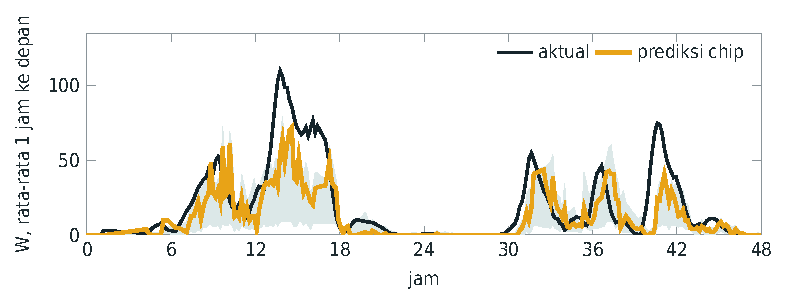
\includegraphics[width=0.9\linewidth]{../presentasi/hackathon-2026/demo-day/gambar/prediksi.pdf}\end{center}
\textbf{Cara membaca:} garis gelap = aktual, garis kuning = prediksi chip, area muda = rentang 80\%. Prediksi mengikuti pola naik-turun harian,
lebih halus dari aktual karena memprediksi \emph{rata-rata} 1 jam. Puncak tajam singkat tidak bisa ditebak tepat oleh model mana pun.

\section{Fitur 2 --- Status turbin dari kurva daya wajar}
Model kedua (MLP INT8 dengan 16 fitur angin/cuaca, tanpa fitur daya) memperkirakan \textbf{daya yang wajar} untuk angin saat ini.
Uji: MAE 2,57 W. Lalu dihitung rasio daya aktual / daya wajar selama 30 menit:
\begin{itemize}
  \item rasio $<$ 0,42 $\to$ \textbf{Di bawah normal} (kemungkinan gangguan: bilah, rem, kabel, generator);
  \item 0,42--1,46 $\to$ \textbf{Normal}; rasio $>$ 1,46 $\to$ \textbf{periksa sensor};
  \item daya wajar $<$ 5 W $\to$ \textbf{Angin lemah} (tidak dinilai).
\end{itemize}
Ambang diambil dari data validasi. Kegunaan kedua: saat PZEM tidak merespons, daya wajar inilah yang mengganti daya yang hilang.
\textbf{Batasan jujur:} uji kerusakan buatan menunjukkan deteksi baik untuk penurunan daya besar (sisa 20\%: 67,5\% jendela terdeteksi, alarm palsu 4\%),
lemah untuk penurunan kecil. Label ``SVM TA'' di dashboard adalah model lama tugas akhir di Raspi (Optimal/Anomaly dari Cp), terpisah dari ini.

\section{Fitur 3 --- Aki 1 jam ke depan (simulasi)}
Prediksi fitur 1 dimasukkan ke rantai \emph{turbin $\to$ charge controller $\to$ aki $\to$ inverter $\to$ beban}. Asumsi: aki timbal-asam
\textbf{12 V 50 Ah} (600 Wh, dipakai sampai 50\% agar awet), efisiensi isi 0,90 / buang 0,95, beban 6 W ditambah 25 W pukul 18--23. Keluaran:
SoC sekarang dan 1 jam lagi, energi masuk aki, serta peringatan ``perlu PLN''. Kelebihan saat aki penuh dialihkan ke dump load 35\,$\Omega$.
Uji (simulasi Okt): galat SoC 1 jam \textbf{0,66 poin persen} (persistence 1,09); peringatan PLN presisi 96,5\%, recall 92,9\%.
\textbf{Ini masih simulasi}: aki belum terpasang (target Desember 2026).

\section{Mode ketahanan: prediksi tetap ada saat data bermasalah}\label{sec:mode}
\begin{center}
\begin{tikzpicture}[node distance=0.25cm, every node/.style={font=\footnotesize}]
  \node[milik=genis, text width=10.5cm] (a) {\textbf{1. Normal}: $\ge$50 dari 60 menit terakhir berisi data};
  \node[milik=izma, text width=10.5cm, below=of a] (b) {\textbf{2. Data berlubang (celah)}: Raspi reboot singkat; cukup separuh jendela (30 menit)};
  \node[milik=izma, text width=10.5cm, below=of b] (c) {\textbf{3. Offline}: Open-Meteo tidak tersedia $\to$ model INT8 offline};
  \node[milik=alif, text width=10.5cm, below=of c] (d) {\textbf{4. Pemulihan}: Raspi baru kembali setelah mati lama; cukup 3 menit data};
  \node[milik=shania, text width=10.5cm, below=of d] (e) {\textbf{Paralel, PZEM diam}: angin $<$1,4 m/s $\to$ daya 0 W; angin cukup $\to$ daya wajar dari kurva daya};
\end{tikzpicture}
\end{center}
Mesin mencoba urutan 1 $\to$ 4; yang pertama berhasil dipakai. Semua mode diberi label di dashboard (ringkasan satu baris, detail bisa dibuka).

\begin{tabularx}{\linewidth}{@{}>{\raggedright}p{2.3cm} >{\raggedright}X >{\raggedright\arraybackslash}p{6.2cm}@{}}
\toprule
Mode & Uji (data 1--20 Okt) & Hasil \\
\midrule
PZEM diam & daya kosong diganti daya wajar / 0 W (20.997 menit) & MAE 5,14 W vs normal 5,07 W \\
Data berlubang & 20\% menit dibuang secara acak & prediksi ada 97,7\% waktu; MAE 5,07 vs 5,00 W \\
Offline & tanpa prakiraan Open-Meteo & MAE 5,62 vs 5,48 W \\
Pemulihan & Raspi mati 75 menit, berulang tiap 3 jam (5.075 menit) & MAE 6,04 W vs data utuh 5,99 W, persistence 8,73 W; prediksi kembali menit ke-3 \\
\bottomrule
\end{tabularx}

\textbf{Aturan ambang putar (cut-in):} PZEM-017 mati di bawah 7 V (maksimal 7$^2$/35 = 1,4 W). Data menunjukkan PZEM kosong pada 51,5\% menit di
1,3--1,4 m/s dan 98\% di 0,8 m/s; 97,8\% menit kosong terjadi saat angin $<$2 m/s. Maka daya kosong saat angin $<$1,4 m/s dihitung 0 W, sama dengan
aturan data latih. Ini tidak mengubah model, sehingga tidak perlu latih ulang atau flash ulang chip.

\begin{perhatian}[Yang tidak bisa diatasi software]
Selama Raspi benar-benar mati, tidak ada data baru sama sekali sehingga prediksi berhenti; data periode itu hilang permanen (juga di
Google Sheets dan InfluxDB). Solusi produk: Edge Kit membaca sensor dan menghitung prediksi langsung di turbin dengan buffer lokal.
\end{perhatian}

\section{Hubungan dengan chip FPGA}
\begin{itemize}
  \item Fitur INT8 yang sama dikirim ESP32-S3 ke Tang Nano 4K dalam paket UART 19 byte (dengan CRC-8); chip membalas 7 byte. 309 siklus per prediksi.
  \item Karena bobot dan aritmetika identik, dashboard bisa menulis ``\textbf{identik dengan CPU}''. Uji di papan 21 Okt: 5.373/5.373 inferensi sama.
  \item Daya: Raspberry Pi $\approx$2,96 W vs papan chip $\approx$0,17 W; energi per prediksi 182 J vs 10,4 J ($\approx$17$\times$). Estimasi INA219 tanpa
        multimeter pembanding; kanal chip kemungkinan hanya mengukur FPGA.
  \item Model sengaja kecil: inilah alasan bisa muat di chip hemat daya. Model besar (Transformer) hanya sedikit lebih akurat (RMSE 10,07 vs 10,25 W).
\end{itemize}

\section{Membaca panel ML di dashboard}
\begin{tabularx}{\linewidth}{@{}l X@{}}
\toprule
Rata-rata daya 1 jam & prediksi utama (W = Wh jam berikutnya) dan rentang 80\% \\
Energi 1 jam berikutnya & angka yang sama dalam Wh \\
Prakiraan angin (Open-Meteo) & rata-rata angin model cuaca 1 jam ke depan; ini grid cuaca, bukan anemometer atap \\
Akurasi live 24 jam (MAE) & prediksi yang dibuat 60 menit lalu dibandingkan aktual; contoh 22 Okt: 11,5 W vs persistence 23,7 W \\
Baris Chip & ``Tang Nano 4K \ldots{} identik dengan CPU'' bila papan menyala; bila tidak, prediksi tetap dari CPU dengan bobot yang sama \\
Keterangan mode & satu baris ringkas; ``detail'' membuka penjelasan dan angka uji \\
\bottomrule
\end{tabularx}
\textbf{Kenapa akurasi live bisa lebih besar dari uji (5,48 W)?} Galat absolut naik saat angin kencang (daya besar dan berubah cepat);
yang penting model tetap jauh lebih baik dari persistence pada hari yang sama. Hari tenang galatnya kecil.

\section{Batasan yang perlu disampaikan dengan jujur}
\begin{itemize}
  \item Baru satu turbin, satu lokasi. Untuk turbin/iklim lain model perlu dilatih ulang dengan data lokasi itu (pilot 2027).
  \item Angin stasiun tidak tepat di rotor; Open-Meteo adalah grid cuaca, bukan pengukuran atap.
  \item Aki dan inverter masih simulasi. Daya INA219 belum dibandingkan multimeter.
  \item Sensor angin error saat hujan (bacaan $>$4 m/s dengan PZEM kosong); belum difilter khusus.
  \item ``OFF'' di Sheet tidak selalu berarti turbin berhenti (bisa juga bacaan PZEM belum masuk saat baris ditulis).
\end{itemize}
\textbf{Rencana:} status \cmd{tegangan\_rendah} vs \cmd{sensor\_error} dari pembaca sensor; model dua tahap (``berputar atau tidak'' lalu
``berapa dayanya''), yang perlu latih ulang lalu bobot baru di Node-RED, ESP32, dan FPGA (sintesis + flash), diuji paritas dan HIL.

\section{Bank pertanyaan juri dan jawaban}
\begin{jawab}[1. Kenapa prediksi 1 jam, bukan 1 hari?]
Keputusan aki, beban, dan PLN dibuat dalam hitungan jam. Untuk turbin kecil, 1 jam cukup untuk bertindak dan masih bisa diprediksi
dengan baik; prediksi harian lebih bergantung pada model cuaca.
\end{jawab}
\begin{jawab}[2. Datanya dari mana? Sintetis?]
Data nyata turbin atap CRIMSE ITB, 181.228 menit (Mar--Okt 2026), plus arsip Open-Meteo. Tidak ada data sintetis untuk melatih model.
\end{jawab}
\begin{jawab}[3. Bagaimana tahu modelnya bagus, bukan kebetulan?]
Dibagi menurut waktu: latih Mar--Jul, pilih model Agu--Sep, uji 1--20 Okt yang tidak pernah dilihat. Dibandingkan dengan persistence
(acuan standar prakiraan): MAE 5,48 vs 8,67 W ($-$37\%), skill +0,40. Juga dibandingkan 36 metode lain.
\end{jawab}
\begin{jawab}[4. Kenapa tidak pakai deep learning yang lebih canggih?]
Sudah dicoba (LSTM, GRU, TCN, CNN, Transformer). Transformer terbaik hanya sedikit lebih baik (RMSE 10,07 vs 10,25 W) tetapi butuh
komputer besar. MLP INT8 kami muat di chip FPGA kecil dengan daya jauh lebih rendah.
\end{jawab}
\begin{jawab}[5. Apa itu INT8 dan kenapa tidak turun akurasinya?]
Semua angka disimpan sebagai bilangan bulat 8-bit agar hemat di chip. Model dilatih langsung dengan aritmetika itu (QAT), jadi tidak
ada penurunan: QAT 5,48 W, sementara membulatkan model biasa memberi 6,75 W.
\end{jawab}
\begin{jawab}[6. Kalau internet mati?]
Prediksi tetap jalan; tanpa Open-Meteo dipakai model offline (MAE 5,62 vs 5,48 W). Di produk, Edge Kit menghitung di turbin tanpa internet.
\end{jawab}
\begin{jawab}[7. Kalau sensor daya mati?]
Daya diganti daya wajar dari angin (model kurva daya); saat angin di bawah 1,4 m/s dihitung 0 W karena PZEM memang mati di bawah 7 V.
Uji: MAE 5,14 W vs normal 5,07 W.
\end{jawab}
\begin{jawab}[8. Kalau Raspi mati, harus menunggu 1 jam?]
Tidak lagi. Mode pemulihan memprediksi 3 menit setelah data kembali; uji Raspi mati 75 menit: MAE 6,04 W, hampir sama dengan data utuh 5,99 W.
\end{jawab}
\begin{jawab}[9. Apakah model belajar terus saat live?]
Tidak. Bobot tetap (sama dengan di chip), dilatih ulang terkendali di laptop bila ada data baru, lalu dipasang serentak di Node-RED, ESP32, dan FPGA
setelah lulus uji kesamaan. Ini disengaja supaya hasil chip selalu bisa diverifikasi.
\end{jawab}
\begin{jawab}[10. Bisa untuk turbin lain atau banyak turbin?]
Arsitekturnya per turbin (satu Edge Kit per turbin, satu dashboard untuk banyak turbin). Model perlu dilatih ulang dengan data turbin/lokasi
baru; terbukti baru satu turbin, pilot multi-lokasi target 2027.
\end{jawab}
\begin{jawab}[11. Kenapa akurasi live di dashboard lebih besar dari 5,48 W?]
Akurasi live dihitung 24 jam terakhir dan sangat bergantung kondisi angin; hari berangin galat absolut lebih besar. Pada hari yang sama model
tetap jauh lebih baik dari persistence (contoh 11,5 vs 23,7 W).
\end{jawab}
\begin{jawab}[12. Apa bedanya dengan status ``SVM TA'' di dashboard?]
SVM TA adalah model lama tugas akhir di Raspi yang mengklasifikasi Optimal/Anomaly dari Cp; kini memakai angin stasiun. Status kami
memakai kurva daya wajar yang dipelajari dari data, tidak bergantung asumsi diameter rotor.
\end{jawab}
\begin{jawab}[13. Bagaimana memastikan chip benar-benar menghitung, bukan sekadar menyalin CPU?]
Chip menerima fitur INT8 dan membalas hasil plus jumlah siklus (309) lewat paket ber-CRC; uji di papan 5.373 inferensi dibandingkan model acuan,
dan tiap menit live hasil chip dibandingkan CPU. Bila papan dimatikan, baris chip langsung berubah ``belum tersambung''.
\end{jawab}
\begin{jawab}[14. Rentang 80\% itu artinya apa?]
Delapan dari sepuluh kali, nilai sebenarnya jatuh di dalam rentang itu (uji: 83,2\%). Pemilik tahu bukan hanya angka, tetapi juga seberapa yakin.
\end{jawab}

\section{Glosarium}
\begin{tabularx}{\linewidth}{@{}l X@{}}
\toprule
MAE & \emph{mean absolute error}, rata-rata selisih absolut prediksi dan aktual (W) \\
RMSE & akar rata-rata kuadrat galat; lebih menghukum galat besar \\
Persistence & tebakan paling sederhana: 1 jam lagi sama dengan sekarang; acuan standar \\
Skill & seberapa jauh lebih baik dari persistence (0 = sama, +0,40 = 40\% lebih kecil galat kuadratnya) \\
MLP & \emph{multilayer perceptron}, jaringan saraf berlapis sederhana \\
INT8, QAT & bilangan bulat 8-bit; pelatihan yang memperhitungkan pembulatan chip \\
Open-Meteo & layanan prakiraan cuaca terbuka (model cuaca global/regional) \\
PZEM-017 & meteran daya DC yang dibaca Raspi lewat RS-485 \\
Cut-in & kecepatan angin minimal agar turbin mulai menghasilkan daya ($\pm$1,4 m/s di data kami) \\
HIL & \emph{hardware-in-the-loop}, uji model di papan chip sungguhan \\
\bottomrule
\end{tabularx}

\vspace{4pt}
{\footnotesize Sumber angka: \cmd{ml/results/mlp.json}, \cmd{baselines.json}, \cmd{mlp\_offline.json}, \cmd{status\_mlp\_int8.json},
\cmd{status\_anomali.json}, \cmd{baterai\_simulasi.json}, \cmd{kualitas\_data.json}, \cmd{energi\_harian.json}; \cmd{dashboard/wec/model\_bundle.json};
tes \cmd{dashboard/wec/test/test\_tanpa\_pzem.js}, \cmd{test\_celah.js}, \cmd{test\_pemulihan.js}; \cmd{docs/demo/hil-2026-10-21.txt};
\cmd{docs/presentasi/hackathon-2026/demo-day/cek-angka.md}.}

\end{document}
